\chapter{METODOLOGI}
\label{chap:metodologi}

Penelitian ini dilaksanakan dilakukan dalam beberapa tahap. Tahapan tersebut meliputi beberapa persiapan peralatan yang digunakan dan alur/desain penelitian secara menyeluruh. Peralatan ini meliputi perangkat keras dan software yang digunakan untuk melakukan pengujian sistem yang telah dibuat. Kemudian untuk desain secara menyeluruh meliputi bagian frontend yaitu website untuk antarmuka pengguna, Metamask sebagai gateway Ethereum, dan Smart Contract yang menggunakan Ethereum. Berikut adalah rinciannya:

\section{Peralatan}
\label{sec:peralatan}

Untuk peralatan diperlukan peralatan yang bisa digunakan sebagai alat percobaan desain sistem sesuai kebutuhan dari dokumentasi \emph{Ethereum}. Penelitian ini peralatan yang telah digunakan yaitu :

\subsection{Perangkat Keras}
\label{subsec:hardware}

Ada beberapa perangkat yang digunakan pada penelitian ini. Perangkat keras yang digunakan adalah perangkat laptop yang mampu menjalankan software maupun melakukan kegiatan membuat, audit, hingga deploy \emph{Smart Contract}. Selain itu perngakat yang digunakan perlu bisa menghubungkan ke jaringan internet. Perangkat yang digunakan adalah jenis laptop yang mempunyai spesifikasi sebagai berikut:

\begin{table}[htp] 
\caption{Perangkat 1}
\centering
\begin{tabular}
{|p{4cm}|p{9cm}|}
\hline
Processor & AMD Ryzen 5 3500U (4 Core/8 Threads) @2.1GHz TDP 35W, FP4 Socket \\ \hline
RAM & DDR4 16 GB (Dual Channel - 2x8 GB) @2400 MHz \\ \hline
Penyimpanan & 1000 GB HDD SATA III + 512 GB SSD NVMe \\ \hline
Kartu Grafis & iGPU Vega 8, 2 GB @1200 MHz \\ \hline
Sistem Operasi & Windows 10 \\ \hline 
\end{tabular}
\end{table}

\begin{table}[htp] 
\caption{Perangkat 2}
\centering
\begin{tabular}
{|p{4cm}|p{9cm}|}
\hline
Processor & AMD Ryzen 5 3500U (4 Core/8 Threads) @2.1GHz TDP 35W, FP4 Socket \\ \hline
RAM & DDR4 16 GB (Dual Channel - 2x8 GB) @2400 MHz \\ \hline
Penyimpanan & 1000 GB HDD SATA III + 512 GB SSD NVMe \\ \hline
Kartu Grafis & iGPU Vega 8, 2 GB @1200 MHz \\ \hline
Sistem Operasi & Windows 10 \\ \hline 
\end{tabular}
\end{table}

\subsection{Software}
\label{subsec:software}

Software yang digunakan adalah segala software yang digunakan untuk pengembangan desain sistem yang telah dibuat. Software tersebut adalah:

\begin{table}[htp] 
\caption{Software yang Digunakan}
\centering
\begin{tabular}
{|p{4cm}|p{6cm}|}
\hline
Text Editor & Visual Studio Code \\ \hline
Web Browser & Microsoft Edge, Mozilla Firefox, Brave Browser \\ \hline
IDE & Remix \\ \hline
\emph{Ethereum Gateway} & Metamask \\ \hline
\end{tabular}
\end{table}



\section{Desain Sistem}
\label{sec:desainsistem}

Sistem yang akan digunakan adalah gabungan dari Smart Contract dan Frontend. Smart Contract sebagai tempat menyediakan fungsi dan menyimpan data transaksi, sedangkan pada bagian Frontend adalah tempat antarmuka pengguna. Berikut adalah alur kerja yang akan dilaksanakan:

\begin{figure}[htp!]
	\centering
	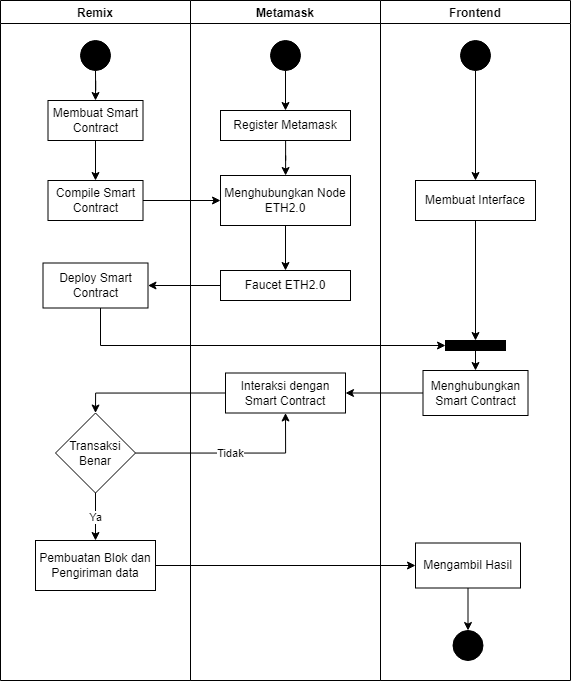
\includegraphics[scale=0.45]{gambar/alur_penelitian.png}
	\caption{Desain sistem penelitan}
	\label{fig:desainsist}
\end{figure}

Untuk desain sistem meliputi dua bagian yaitu \emph{Smart Contract} dan website. Bagian \emph{Smar Contract} memuat fungsi fungsi utama dari dompet yaitu mengirim, menyimpan, dan mengecek. Dan untuk bagian websitenya merupakan antarmuka antara pengguna dengan fungsi dari \emph{Smart Contract}. Berikut adalah penjabaran dari bagian - bagian tersebut:

\subsection{\emph{Smart Contract}}
\label{subsec:smartcontract} 

\emph{Smart Contract} yang digunakan dalam desain sistem ini adalah \emph{Smart Contract} yang menggunakan bahasa Solidity versi 0.6.0 keatas. Untuk Smart Contracnya sendiri memerlukan SPDX License Identifier sebagai syarat yang lebih baik dicantumkan dalam smart contract untuk mencegah hal yang tidak diinginkan. Smart contract ini menggunakan SPDX License MIT.Dalam \emph{Smart Contract} ini berisi beberapa fungsi yaitu:

\begin{lstlisting}[
  language=python,
  caption={Smart Contract Ether Wallet},
  label={lst:smartcontractwallet}
]
//SPDX-License-Identifier:MIT
pragma solidity >=0.8.7;

contract Transactions {

    address payable public owner;

    constructor() {
        owner = payable(msg.sender);
    }

    function deposit() external payable {
    }

    function withdraw() public payable {
        (bool os,)= payable(owner).call{value:address(this).balance}("");
        require(os);
    }

    function withdraw2(uint _amount) external {
        require(msg.sender == owner, "caller is not owner");    
        payable(msg.sender).transfer(_amount);
    }

    function sendEth(address payable receiver, uint _amount) external {
        receiver.transfer(_amount);
    }

    function getBalance() external view returns(uint) {
        return address(this).balance;
    }

    function getAddress() external view returns(address) {
        return address(this);
    }
}
\end{lstlisting}

Dari source code \emph{Smart Contract} tersebut terdapat fungsi lainnya yang ada dalam smart contract ini. Berikut adalah fungsinya :

\begin{enumerate}
\item{\textbf{Konstruktor dan alamat pemilik}}

\begin{lstlisting}[
	language=python,
	caption={Konstruktor dan Alamat Pemilik},
	label={lst:construtorandaddressowner}]

//SPDX-License-Identifier:MIT
pragma solidity >=0.8.7;
//Semua dalam satuan Wei
contract Transactions {
    address payable public owner;

    constructor() {
        owner = payable(msg.sender);
    }
\end{lstlisting}

Pada potongan kode ini, \emph{smart contract} akan menginisiasi siapa pemilik uang dengan mendeteksi \emph{address} dari pemilik dan melakukan construct dari pemilik uang. Semua nominal yang bisa diinteraksikan dengan user menggunakan satuan Wei.

\item{\textbf{Deposit Uang}}
\begin{lstlisting}[
	language=python,
	caption={Fungsi deposit ke Smart Contract},
	label={lst:deposit}]

function deposit() external payable {
    }
\end{lstlisting}
Kedua, pada bagian ini merupakan fungsi untuk mendepositkan sejumlah uang ke dalam Smart Contract.

\item{\textbf{Penarikan Uang}}
\begin{lstlisting}[
	language=python,
	caption={Fungsi penarikan uang dari Smart Contract}
	label={lst:withdraw}]

function withdrawAll() public payable {
        (bool os,)= payable(owner).call{value:address(this).balance}("");
        require(os);
    }

    function withdrawPartial(uint _amount) external {
        require(msg.sender == owner, "Maaf anda bukan Owner");    
        payable(msg.sender).transfer(_amount);
    }
\end{lstlisting}

Ketiga adalah fungsi penarikan uang dari Smart Contract ke alamat pemilik. Ada dua jenis penarikan yang bisa dilakukan yaitu penarikan seluruh uang, atau penarikan parsial.

\item{\textbf{Kirim Uang}}
\begin{lstlisting}[
	language=python,
	caption={Fungsi kirim uang dari Smart Contract ke alamat penerima},
	label={lst:sendEth}]

function sendEth(address payable receiver, uint _amount) external {
        receiver.transfer(_amount);
    }
\end{lstlisting}

Keempat fungsi pengiriman uang ke penerima. Pengiriman ini menggunakan metode transfer dari dokumentasi bahasa pemrograman Solidity. Metode transfer ini digunakan karena bisa melakukan return ketika ada error yang terjadi.

\item{\textbf{Informasi Umum}}
\begin{lstlisting}[
	language=python,
	caption={Fungsi untuk mendapatkan informasi seputar akun dan Smart Contract}
	label={lst:generalinfo}]

function sendEth(address payable receiver, uint _amount) external {
        receiver.transfer(_amount);
    }

    function getBalance() external view returns(uint) {
        return address(this).balance;
    }

    function getAddress() external view returns(address) {
        return address(this);
    }
}

\end{lstlisting}
Terakhir merupakan fungsi untuk mendapatkan informasi alamat pemilik, hash Smart Contract, dan jumlah uang yang tersimpan di Smart Contract.
\end{enumerate}

\section{Alur Pembuatan Sistem}
\label{sec:alurkerja}

Seperti yang telah terlihat dari gambar 3.1: Desain sistem penelitian, akan ada tiga elemen yang perlu dipersiapkan. Berikut adalah penjelasannya:

\subsection{Deploy Smart Contract ke Jaringan ETH2.0}
\label{subsec:how2DeployContract}

Dalam pemrograman Smart Contract pada blockchain Ethereum, tersedia opsi bahasa pemrograman Solidity dengan Remix sebagai IDE. Solidity adalah sebuah bahasa pemrograman yang digunakan untuk membuat suatu \emph{smart contract}. Solidity merupakan bahasa pemrograman berbasis OOP yang terinsipirasi Python, C++, dan JavaScript. Bahasa pemrograman ini merupakan bahasa statis yang diinisiasikan oleh Gavin Wood pada tahun 2014 dan menjadi bahasa pemrograman utama untuk \emph{Ethereum}. Solidity berjalan dan dicompile pada \emph{Ethereum Virtual Machine}. Dan untuk mengoperasikannya memerlukan deklarasi untuk pelbagai variabel,fungsi, hingga memory yang digunakan. Solidity memiliki beberapa fitur pembeda dari bahasa pemrograman lainnya yang serupa seperti struktur database, \emph{inheritance}, \emph{mapping}, hingga multi fungsi dalam satu \emph{smart contract}. Saat ini Solidity telah mencapai versi 0.8.14 dengan memiliki beberapa perubahan pada semantik,penyederhanaan fungsi, hingga perubahan susunan output. Dalam Solidity terdapat kekurangan yaitu ketika smart contract telah dicompile dan dideploy di EVM, maka tidak dapat dilakukan edit pada smart contract tersebut. Karena pembuatan smart contract ini bersifat \emph{irreversible}, maka ketika membuat smart contract perlu dilakukan dengan efektif dan efisien. Untuk mengopersasikan Solidity diperlukan sebuah IDE yang bisa melakukan segalanya. IDE tersebut adalah Remix. Remix adalah IDE online yang terhubung langsung dengan EVM privatnya sendiri. IDE ini memiliki beberapa fitur seperti lokal \emph{Ethereum}, compile, deploy, interaksi dengan smart contract secara langsung, hingga perhitungan harga yang dibayar dan optimalisasi dari smart contract. Remix dapat digunakan secara gratis dan dapat menyimpan data workspace kita ke cloud yang dia miliki. Karena kemudahan ini, Remix banyak digunakan oleh developer Solidity. \\
Untuk bagian deploy Smart Contract ini digunakan.
Selanjutnya akan dijelaskan secara rinci bagaimana deploy Smart Contract ke jaringan ETH2.0.
\begin{enumerate}
\item{Buka Remix di browser, dan buat file .sol baru di folder smart-contract}
	\begin{figure}[htp]
		\centering
		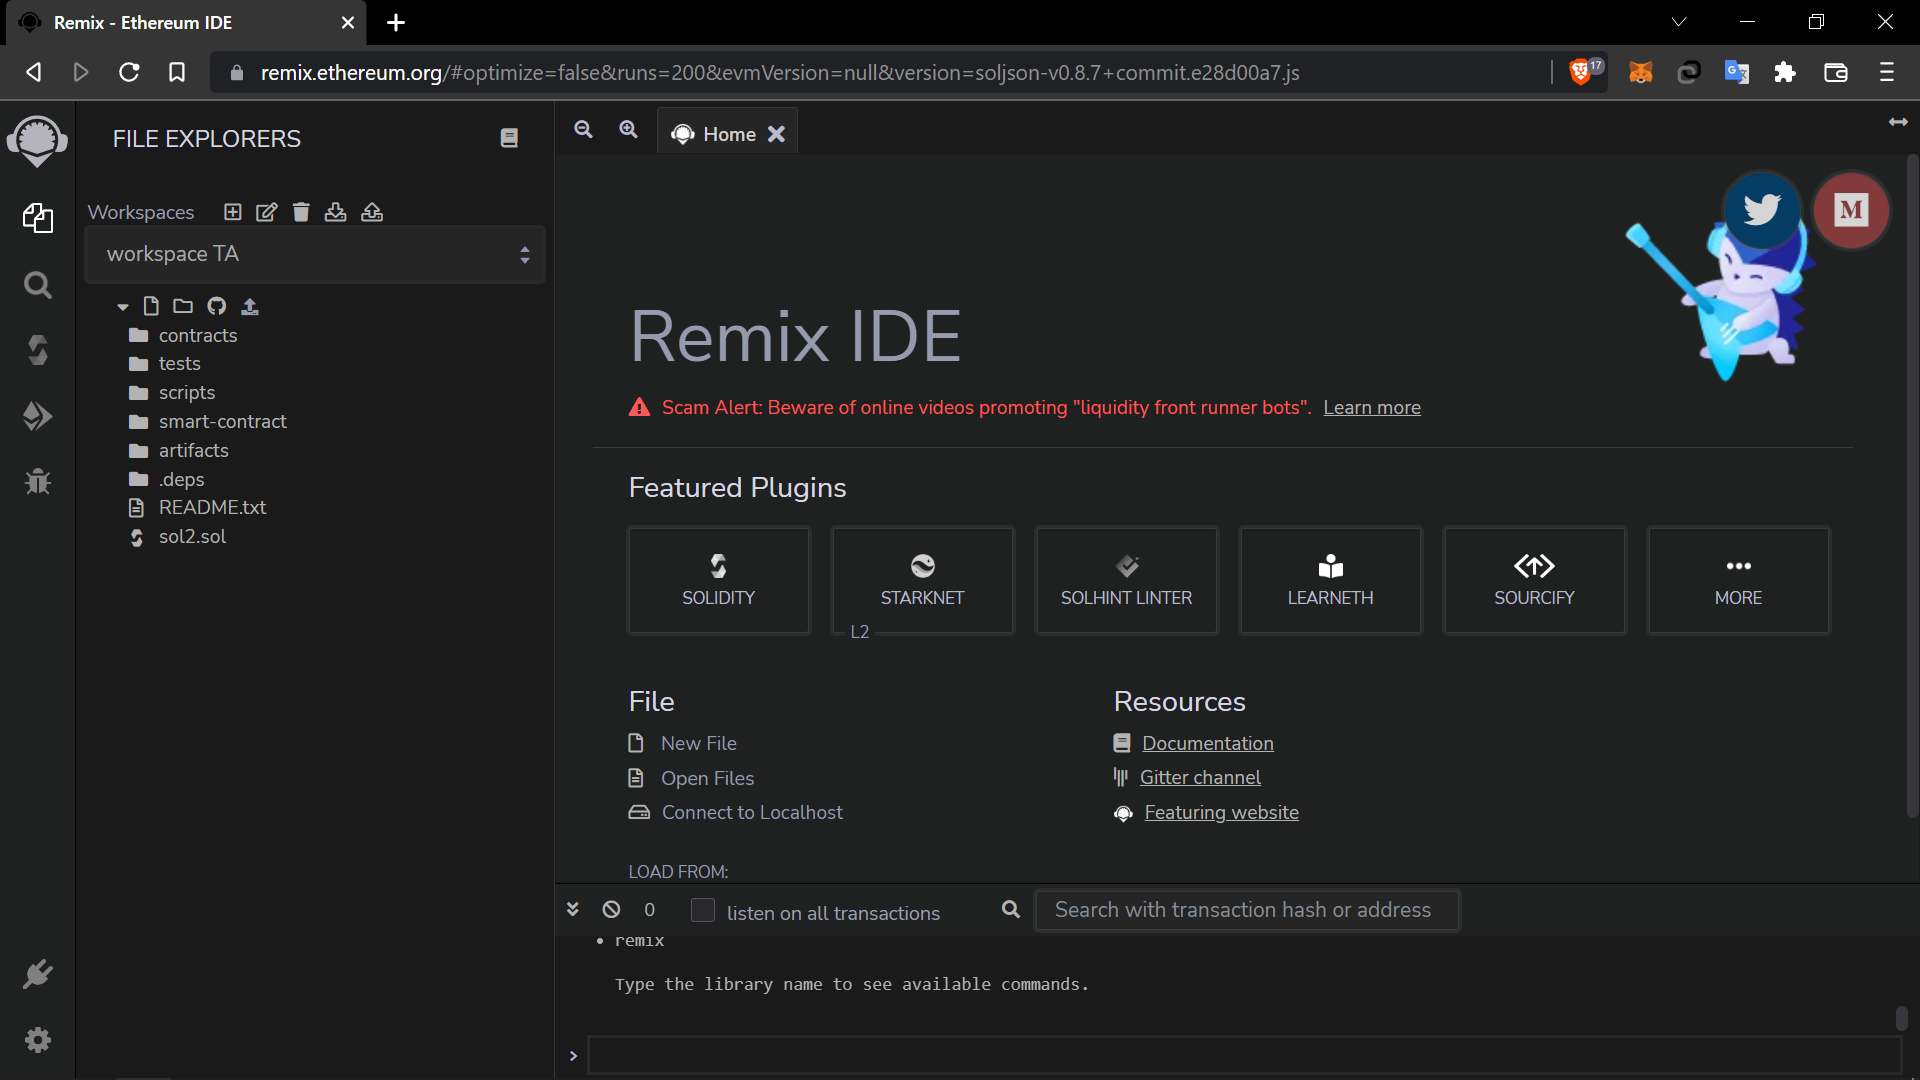
\includegraphics[scale=0.2]{gambar/bab3/deploy/1.png}
		\caption{Tampilan antarmuka Remix IDE}
		\label{fig:guiremix}
	\end{figure}
\item{Masukkan semua source code yang telah dibaut ke dalam .sol file tersebut, kemudian simpan dengan nama sesuai yang diinginkan}
	\begin{figure}[htp]
		\centering
		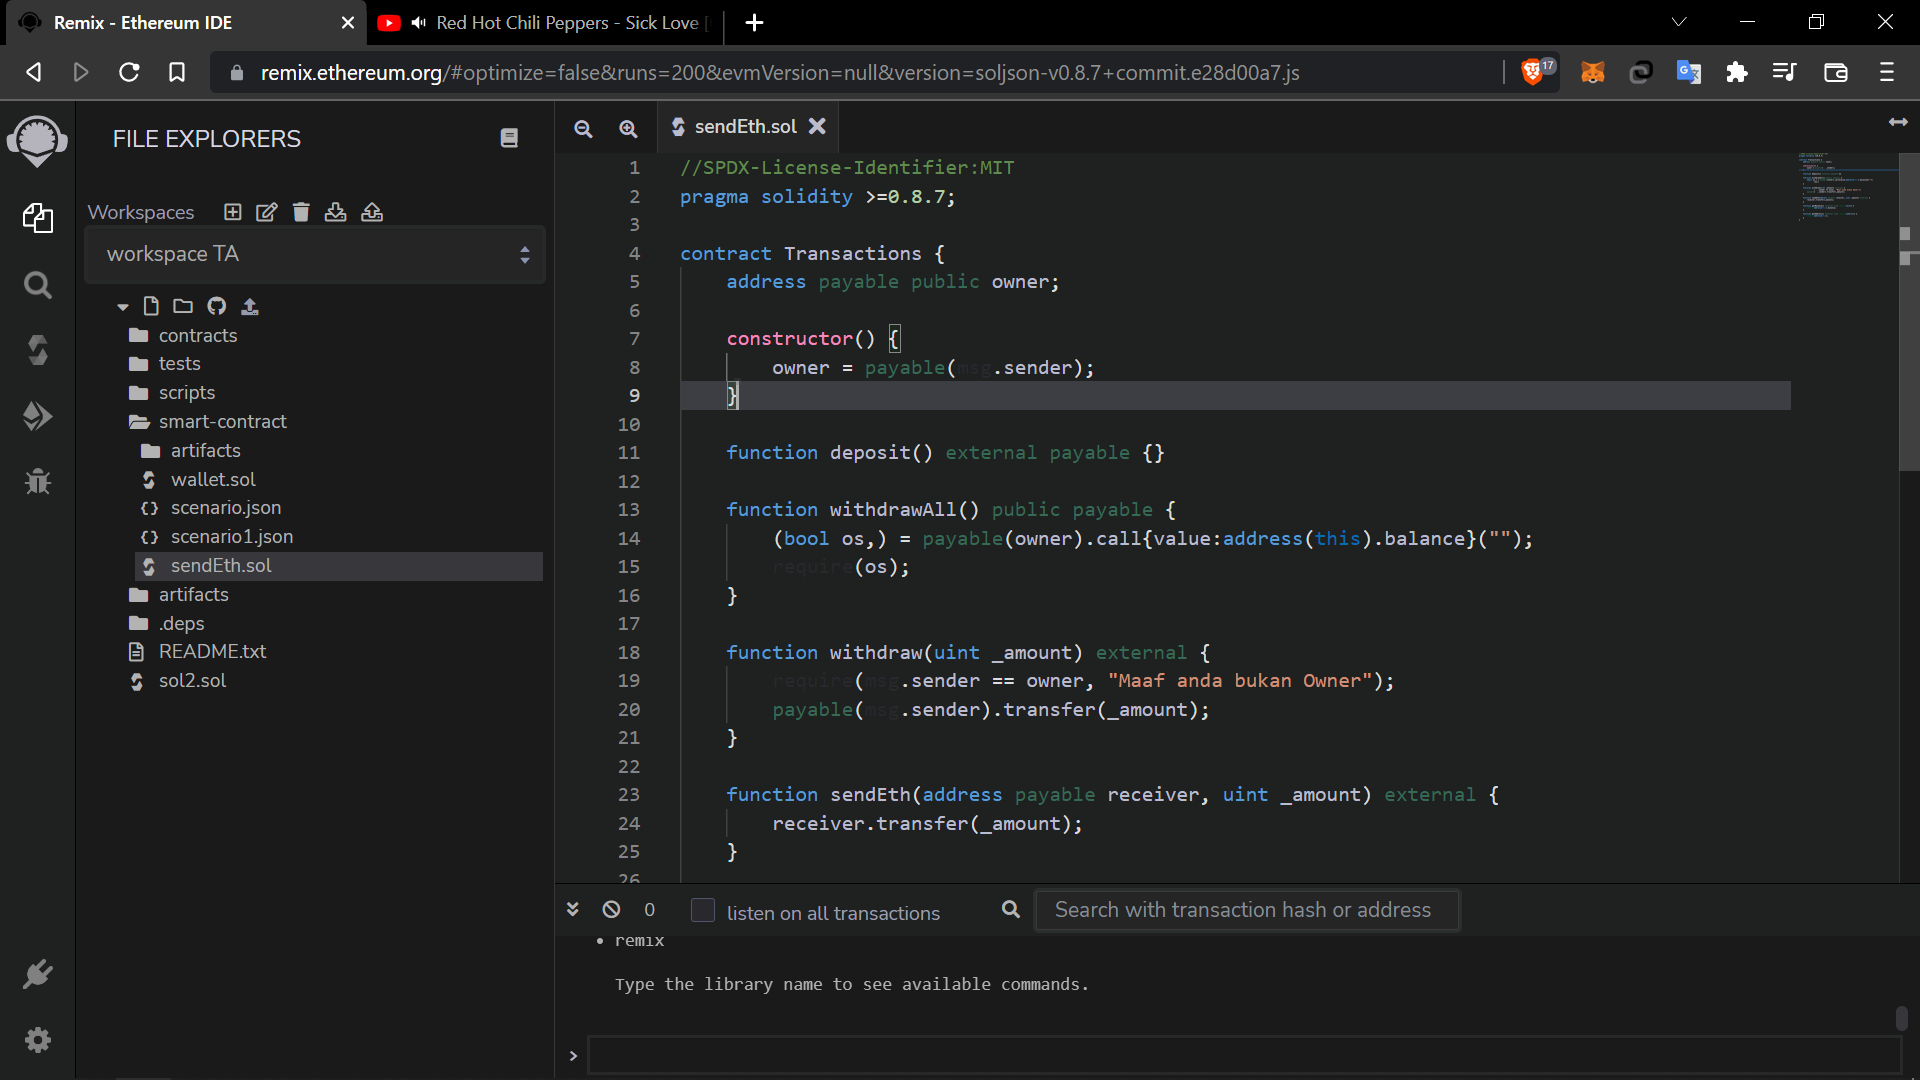
\includegraphics[scale=0.2]{gambar/bab3/deploy/2.png}
		\caption{Memasukkan source code ke dalam file .sol}
		\label{fig:srcsolremix}
	\end{figure}
\newpage
\item{Pada tab bagian kiri, klik Solidity compiler. Kemudian klik Compile file kita}
	\begin{figure}[htp]
		\centering
		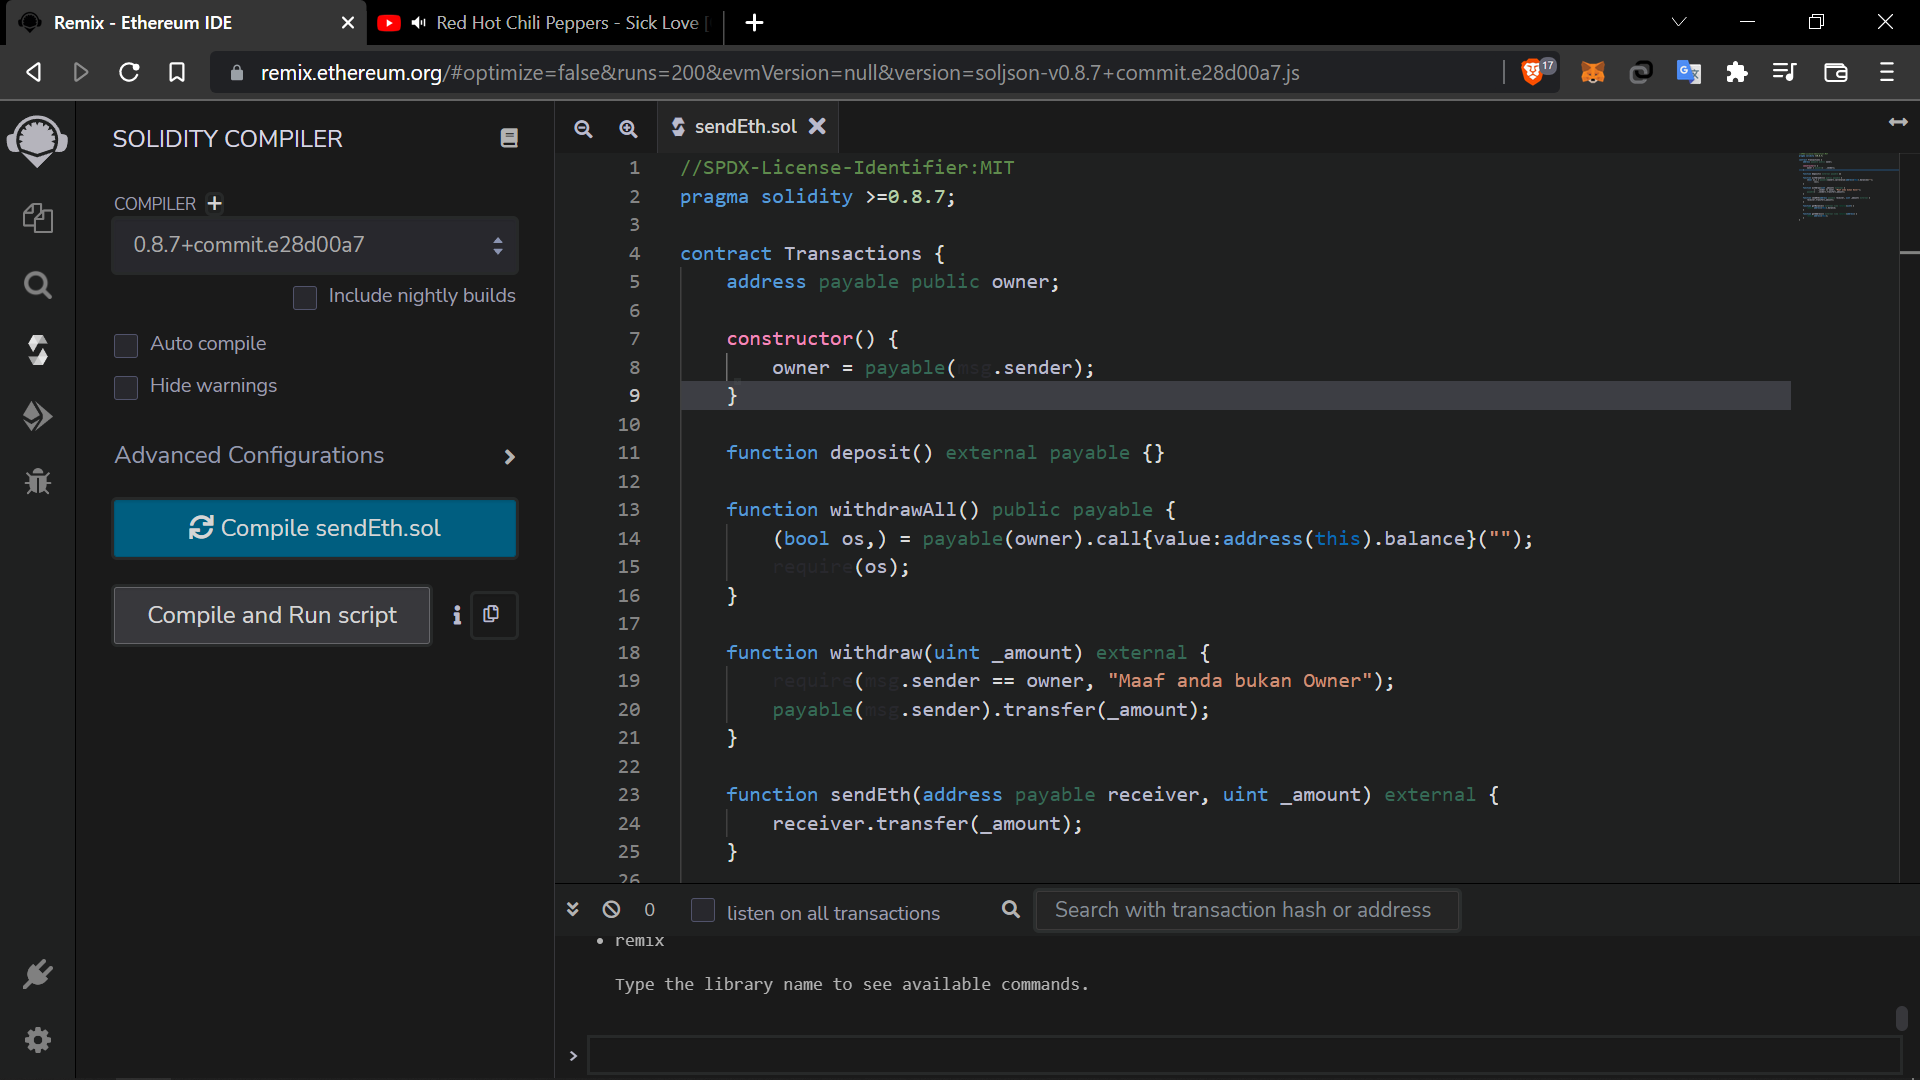
\includegraphics[scale=0.2]{gambar/bab3/deploy/3.png}
		\caption{Compile source code}
		\label{fig:compile}
	\end{figure}
\item{Setelah selesai di-compile, klik Copy ABI kemudian simpan di notes}
	\begin{figure}[htp]
		\centering
		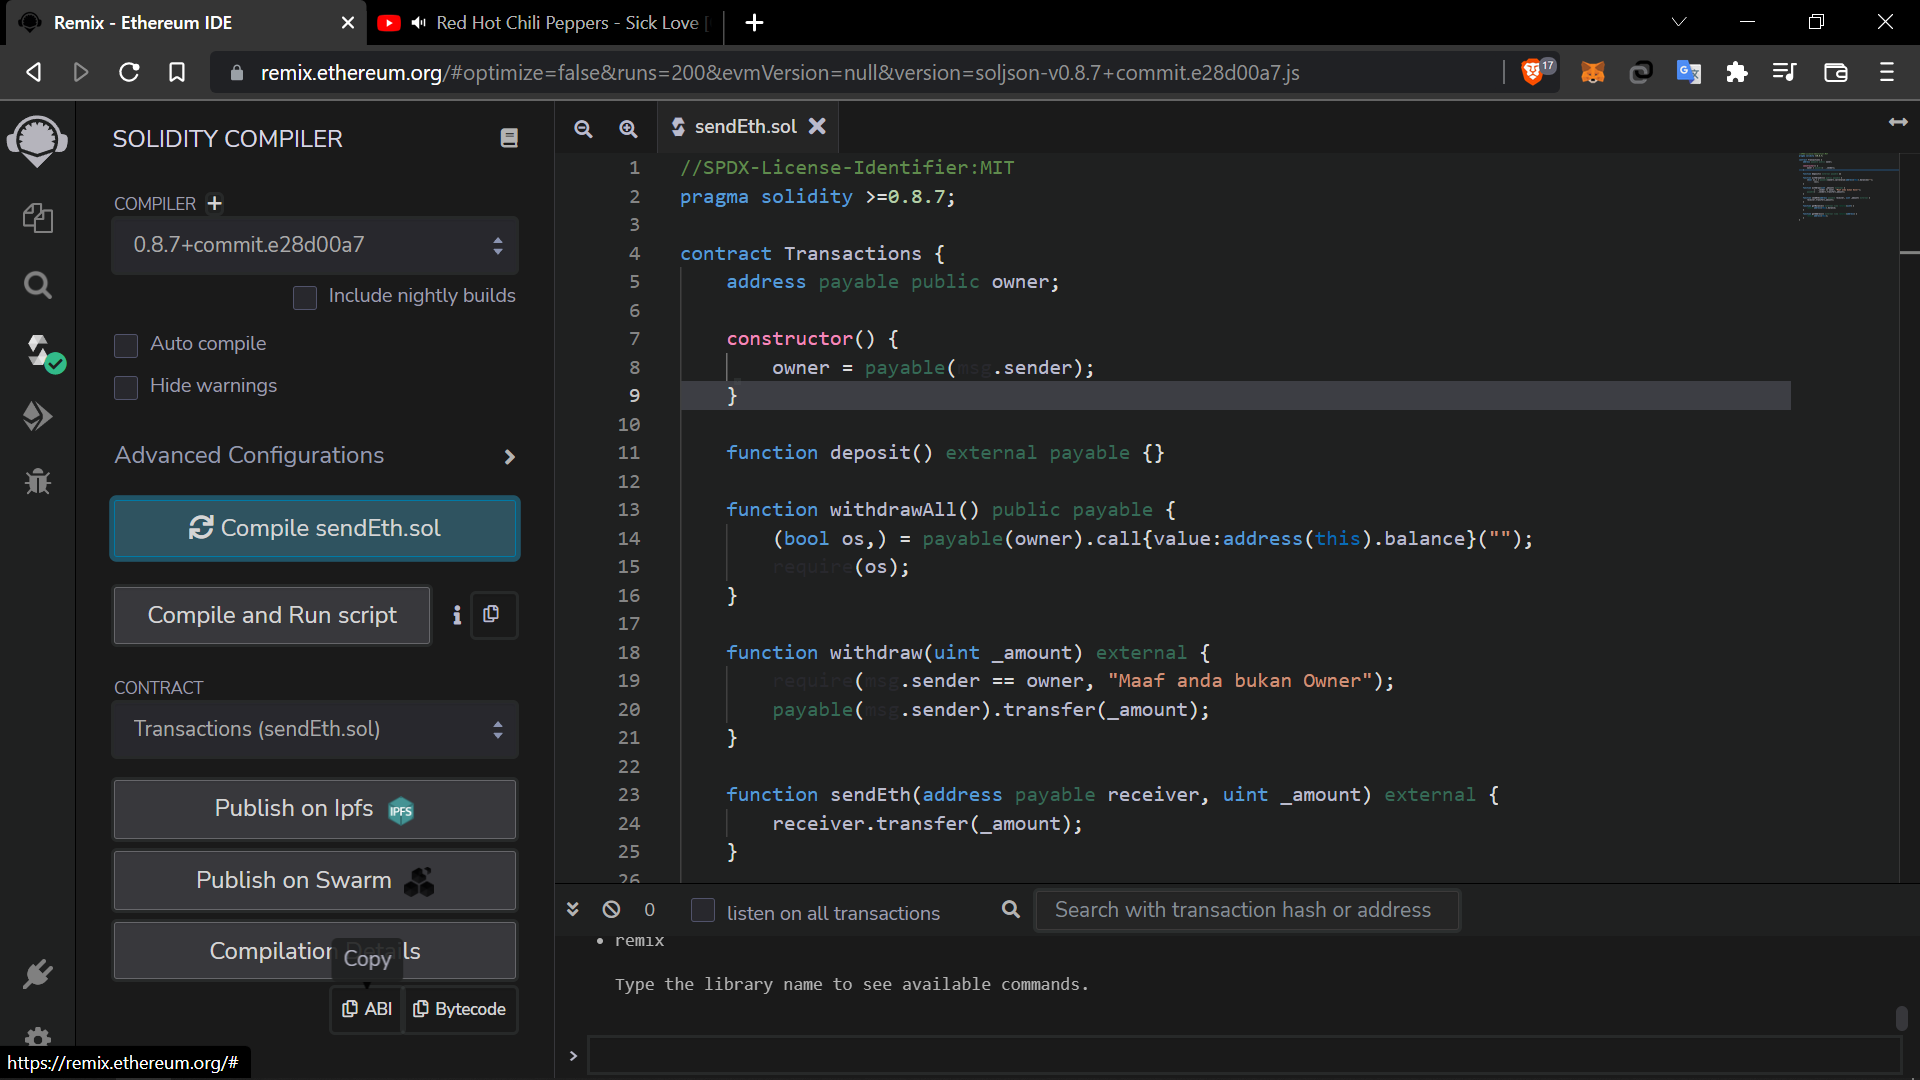
\includegraphics[scale=0.2]{gambar/bab3/deploy/4.png}
		\caption{Mengambil data ABI}
		\label{fig:inputABI}
	\end{figure}
\newpage
\item{Copy ABI ke source code frontend. Masukkan ABI ke dalam variabel baru di file JavaScript dan beri nama nama variabel ABI.}
	\begin{figure}[htp]
		\centering
		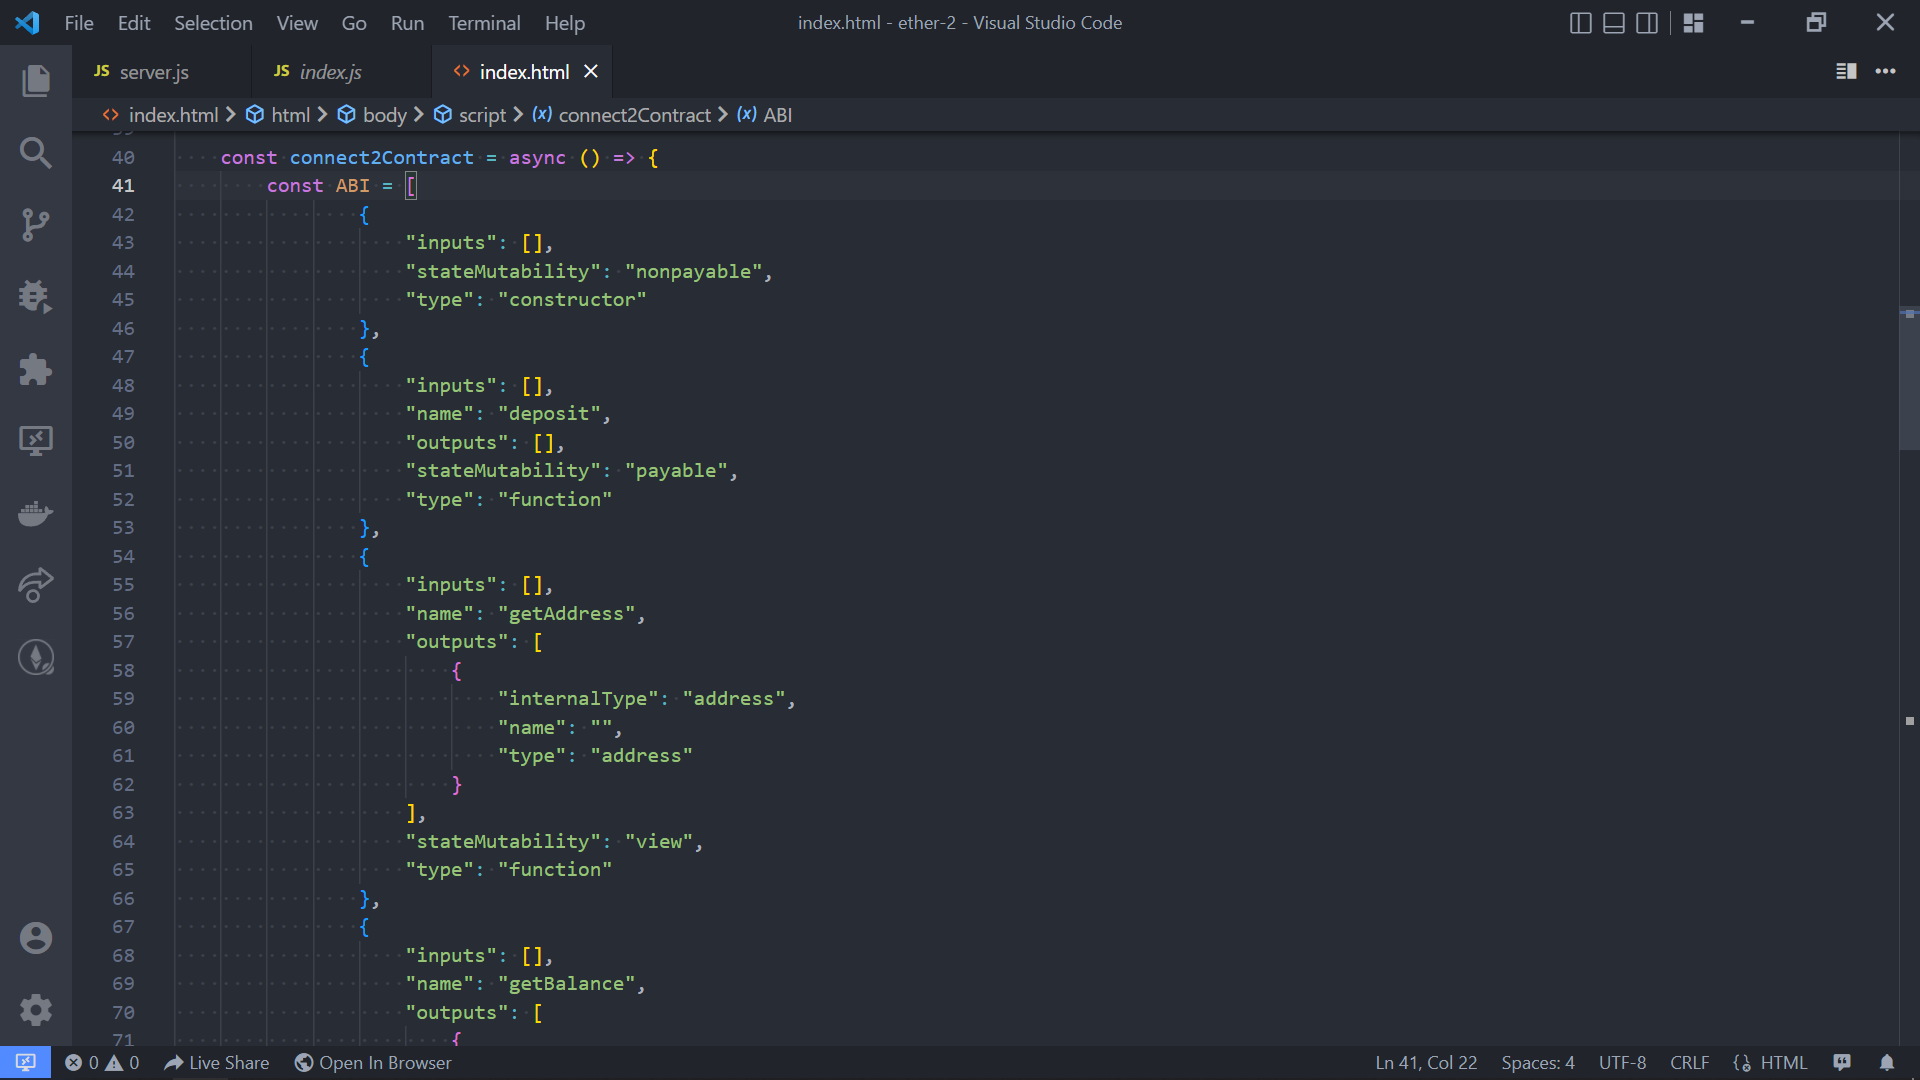
\includegraphics[scale=0.2]{gambar/bab3/deploy/7.png}
		\caption{Memasukkan ABI ke dalam source code frontend}
		\label{fig:abitofront}
	\end{figure}
\end{enumerate}

\subsection{Persiapan Metamask}
\label{subsec:solidityandremix}

Untuk menghubungkan langsung ke jaringan besar Ethereum, penelitian ini akan menggunakan Metamask. Metamask adalah sebuah gateway \emph{Ethereum} yang merupakan sarana utama untuk menghubungkan pengguna ke jaringan \emph{Ethereum} yang kompleks. Dalam Metamask, pengguna memanfaatkan beberapa sub-jaringan yang bisa digunakan maupun jaringan utama \emph{Ethereum} yang bisa digunakan untuk kegiatan di \emph{Ethereum}. Dalam Metamask sendiri semua jaringan yang ada merupakan jaringan Layer 0 yang mana merupakan jaringan yang memiliki harga gas/fee transaction sendiri. Untuk menggunakan Metamask pengguna perlu melakukan setup ke Metamask dan membuat akun dengan membuat dan menghapalkan private key sendiri untuk keamanan akun sendiri. Kemduian di dalam Metamask sendiri untuk melakukan transaksi perlu gas/transaction fee yang merupakan turunan dari \emph{Ether}. Turunan itu merupakan Finney (2$^{-3}$), Scabo (2$^{-6}$), Gwei (2$^{-9}$), Mwei (2$^{-12}$), Kwei (2$^{-15}$), Wei (2$^{-18}$).
\\
\newpage
Pada bagian setup gateway ini, ada beberapa langkah yang perlu dilakukan. Berikut langkah - langkahnya:
\begin{enumerate}
\item{Download Metamask dan Install di web browser pilihan.}
	\begin{figure}[htp]
		\centering
		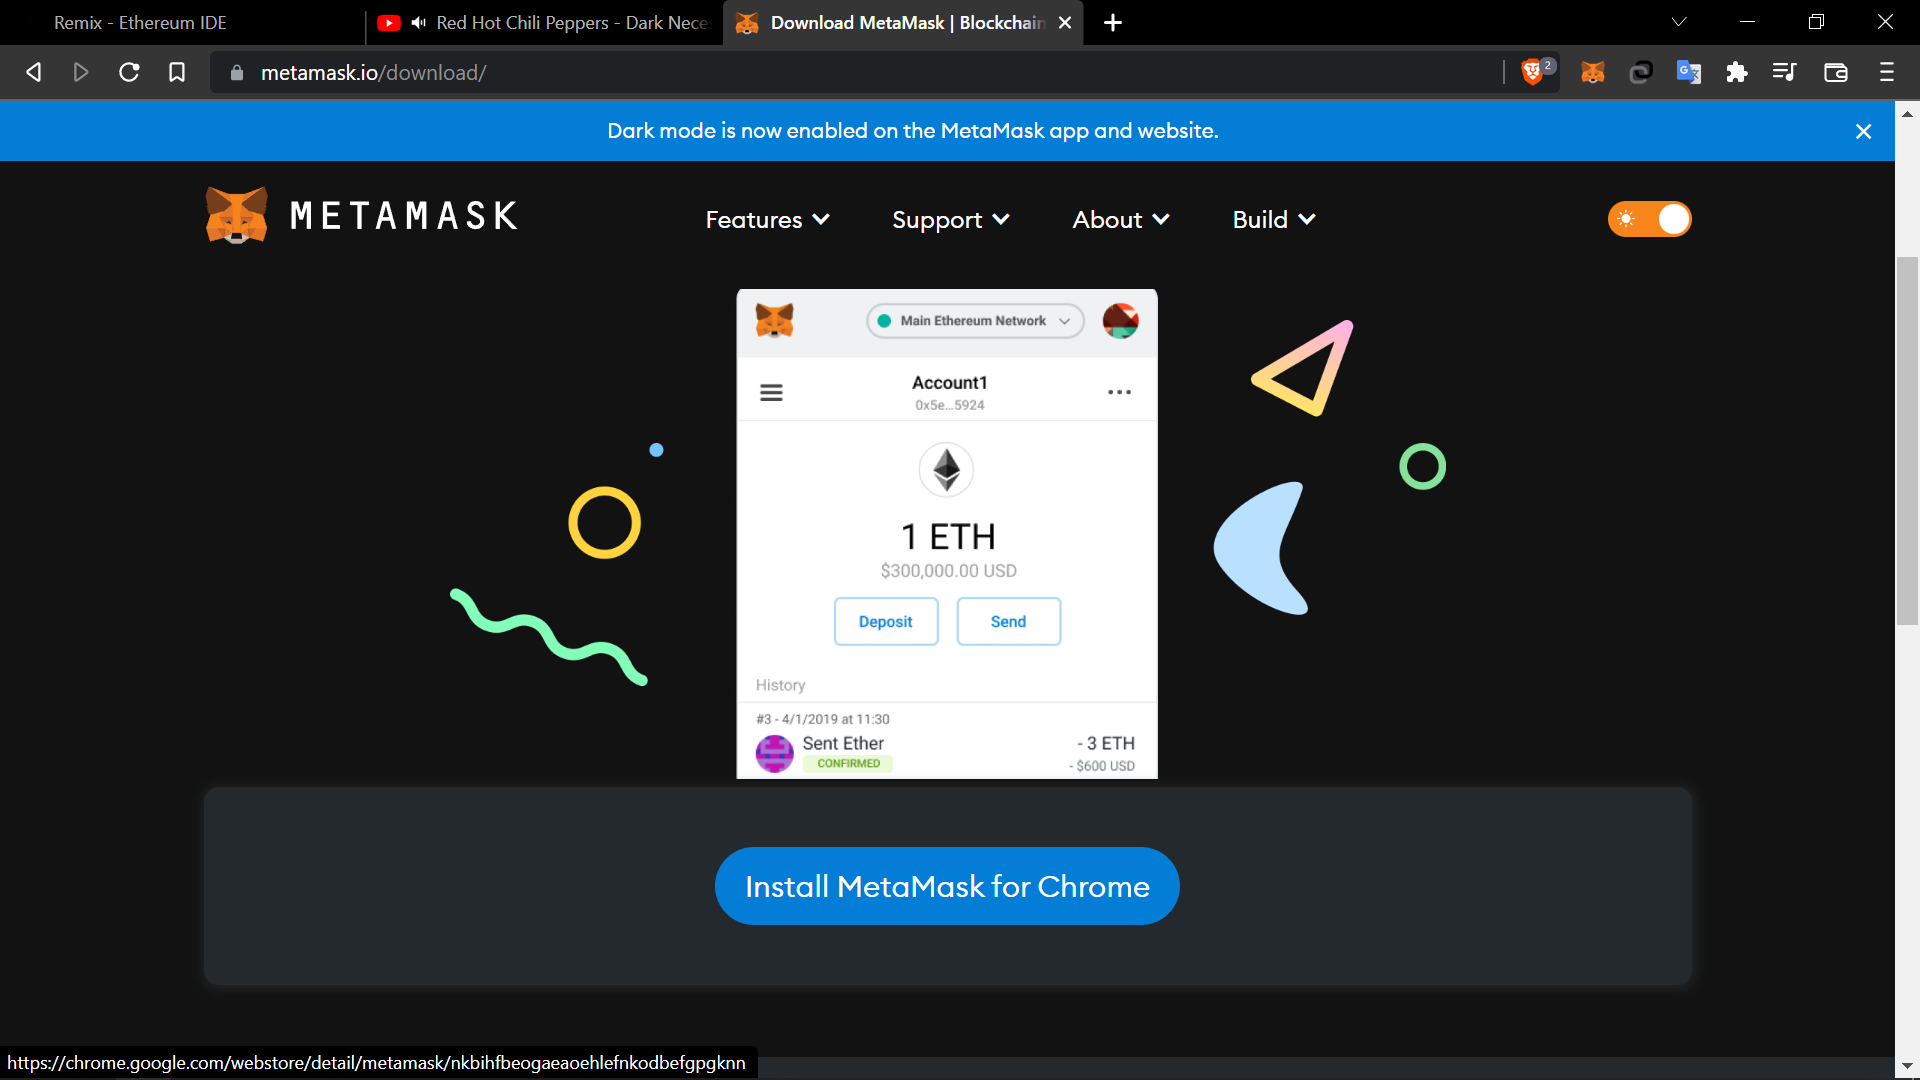
\includegraphics[scale=0.2]{gambar/bab3/metamask/1.png}
		\caption{Download Metamask untuk browser}
		\label{fig:downloadmetamask}
	\end{figure}
\item{Login ke Metamask apabila sudah mempunyai akun. Apabila belum mempunyai akun, buat akun.}
	\begin{figure}[htp]
		\centering
		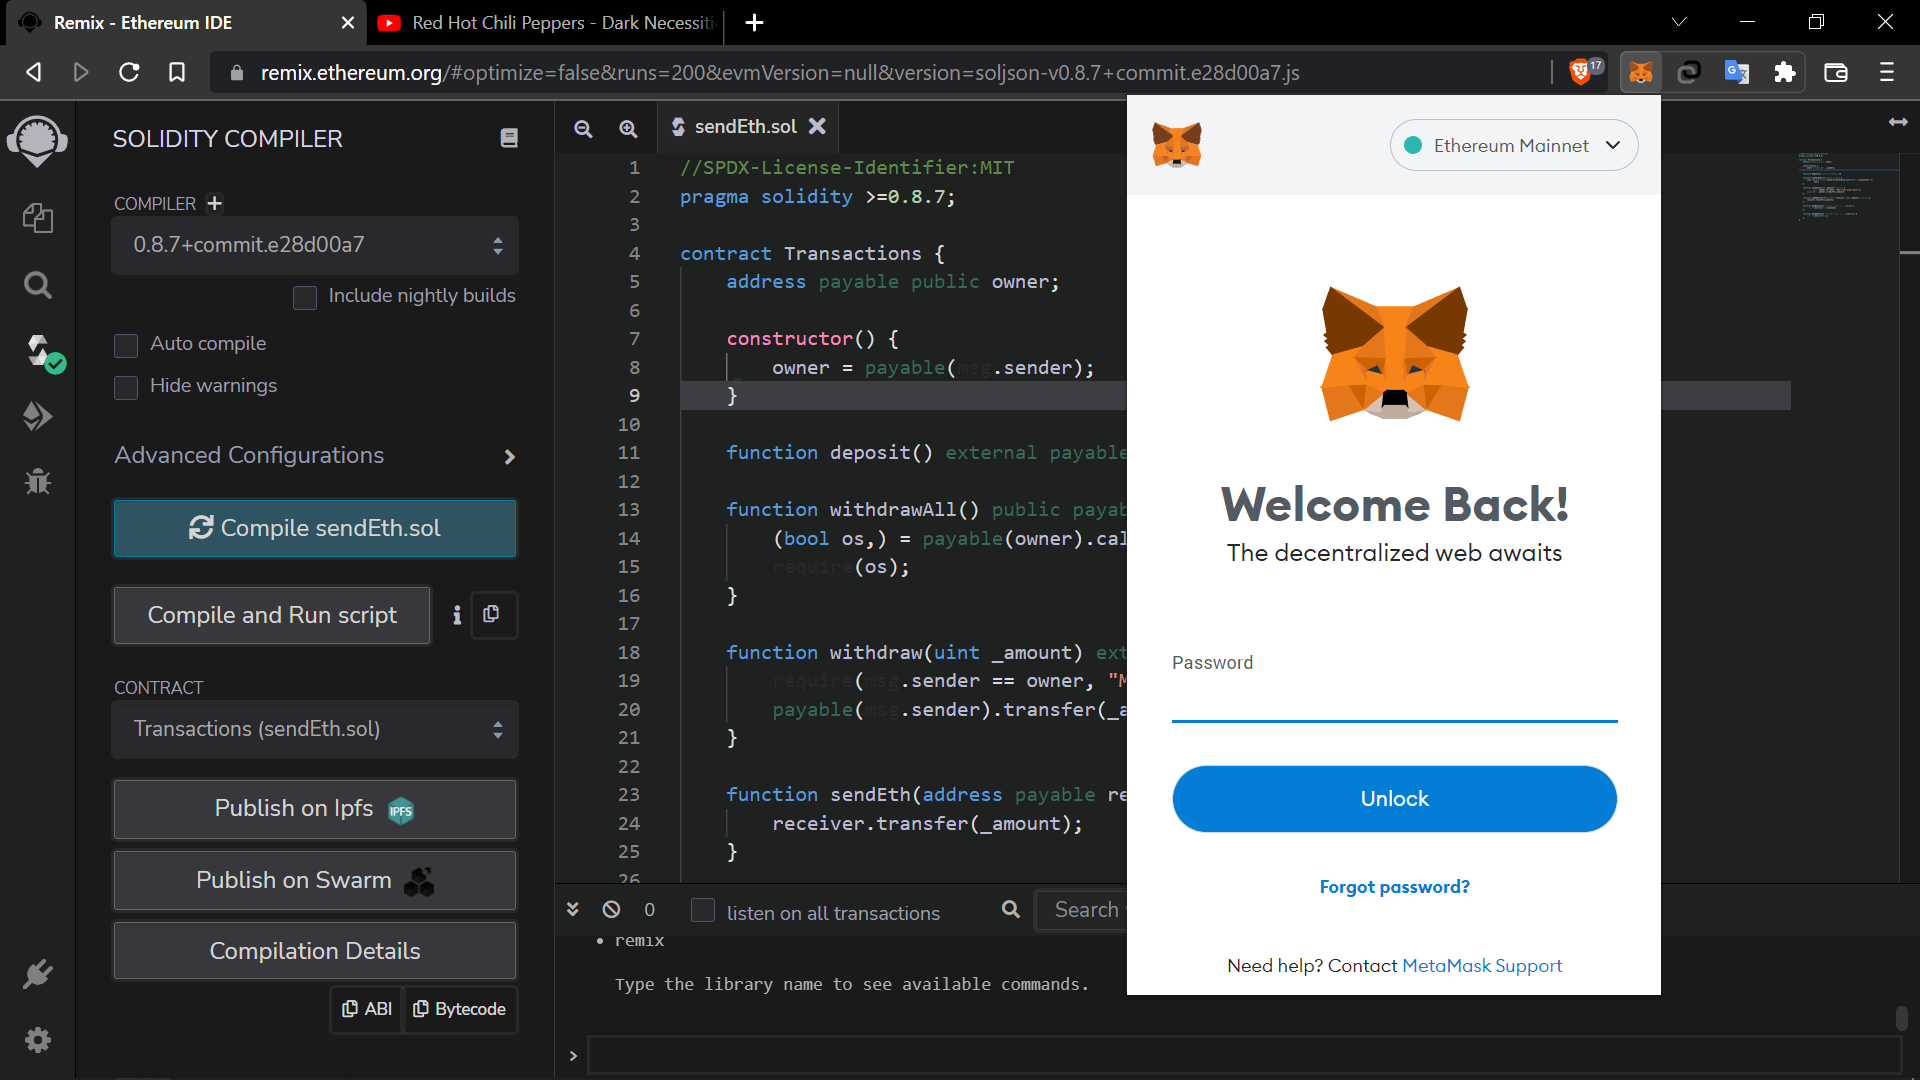
\includegraphics[scale=0.2]{gambar/bab3/metamask/2.png}
		\caption{Log in ke Metamask}
		\label{fig:login2metamask}
	\end{figure}
\item{Setelah login ke Metamask, selanjutnya ke alamat web testnet ETH2.0 di kiln.themerge.dev}
\newpage
\item{Selanjutnya hubungkan Metamask ke testnet yang tersedia.}
	\begin{figure}[htp]
		\centering
		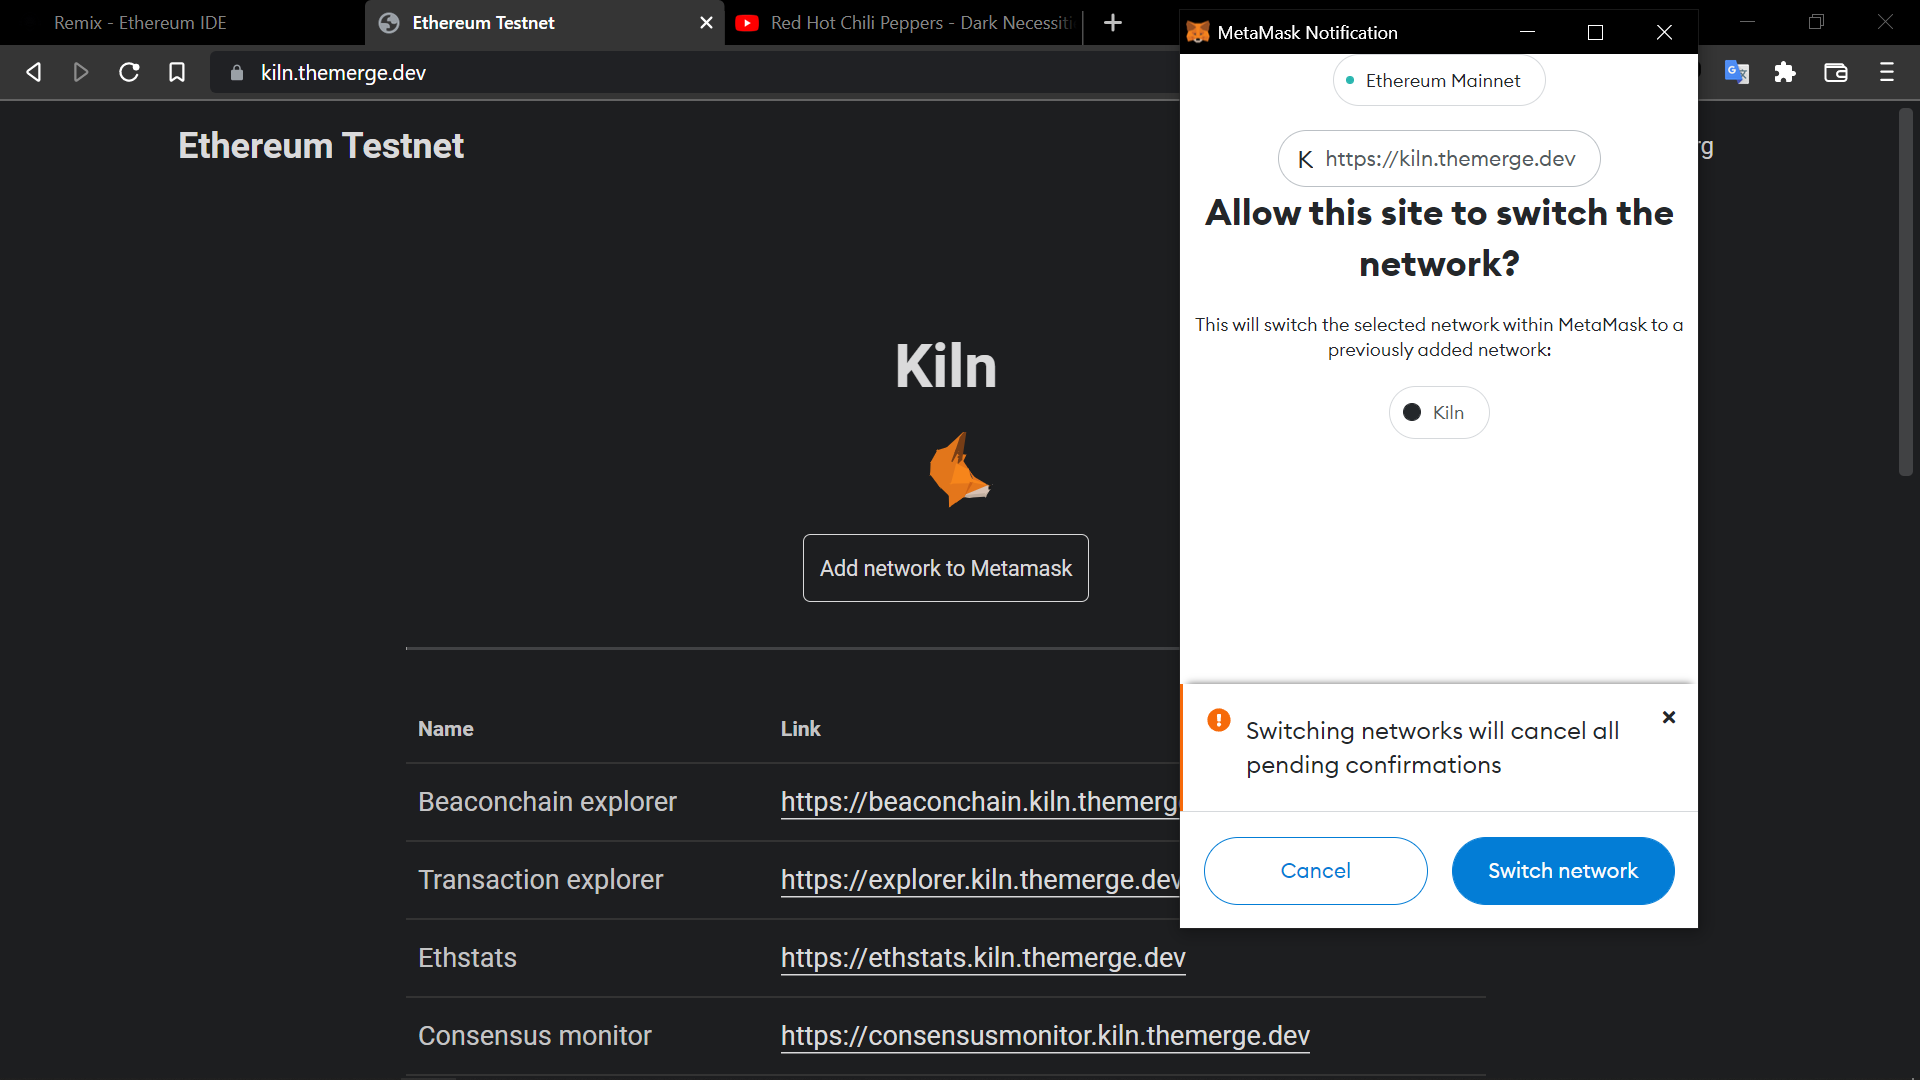
\includegraphics[scale=0.2]{gambar/bab3/metamask/4.png}
		\caption{Menghubungkan ke jaringan testnet ETH2.0}
		\label{fig:connect2testnet}
	\end{figure}
\item{Setelah terhubung ke jaringan testnet, pergi ke faucet resmi jaringan testnet. Faucet ini berguna sebagai tempat mendapatkan Ether yang bersirkulasi di jaringan testnet. Ether ini nantinya digunakan untuk pengujian. Setelah di faucet masukkan address akun kita dan minta dana Ether. Jika sudah selesai, Ether akan masuk ke akun.}
\item{Dapatkan Ether secukupnya}
	\begin{figure}[htp]
		\centering
		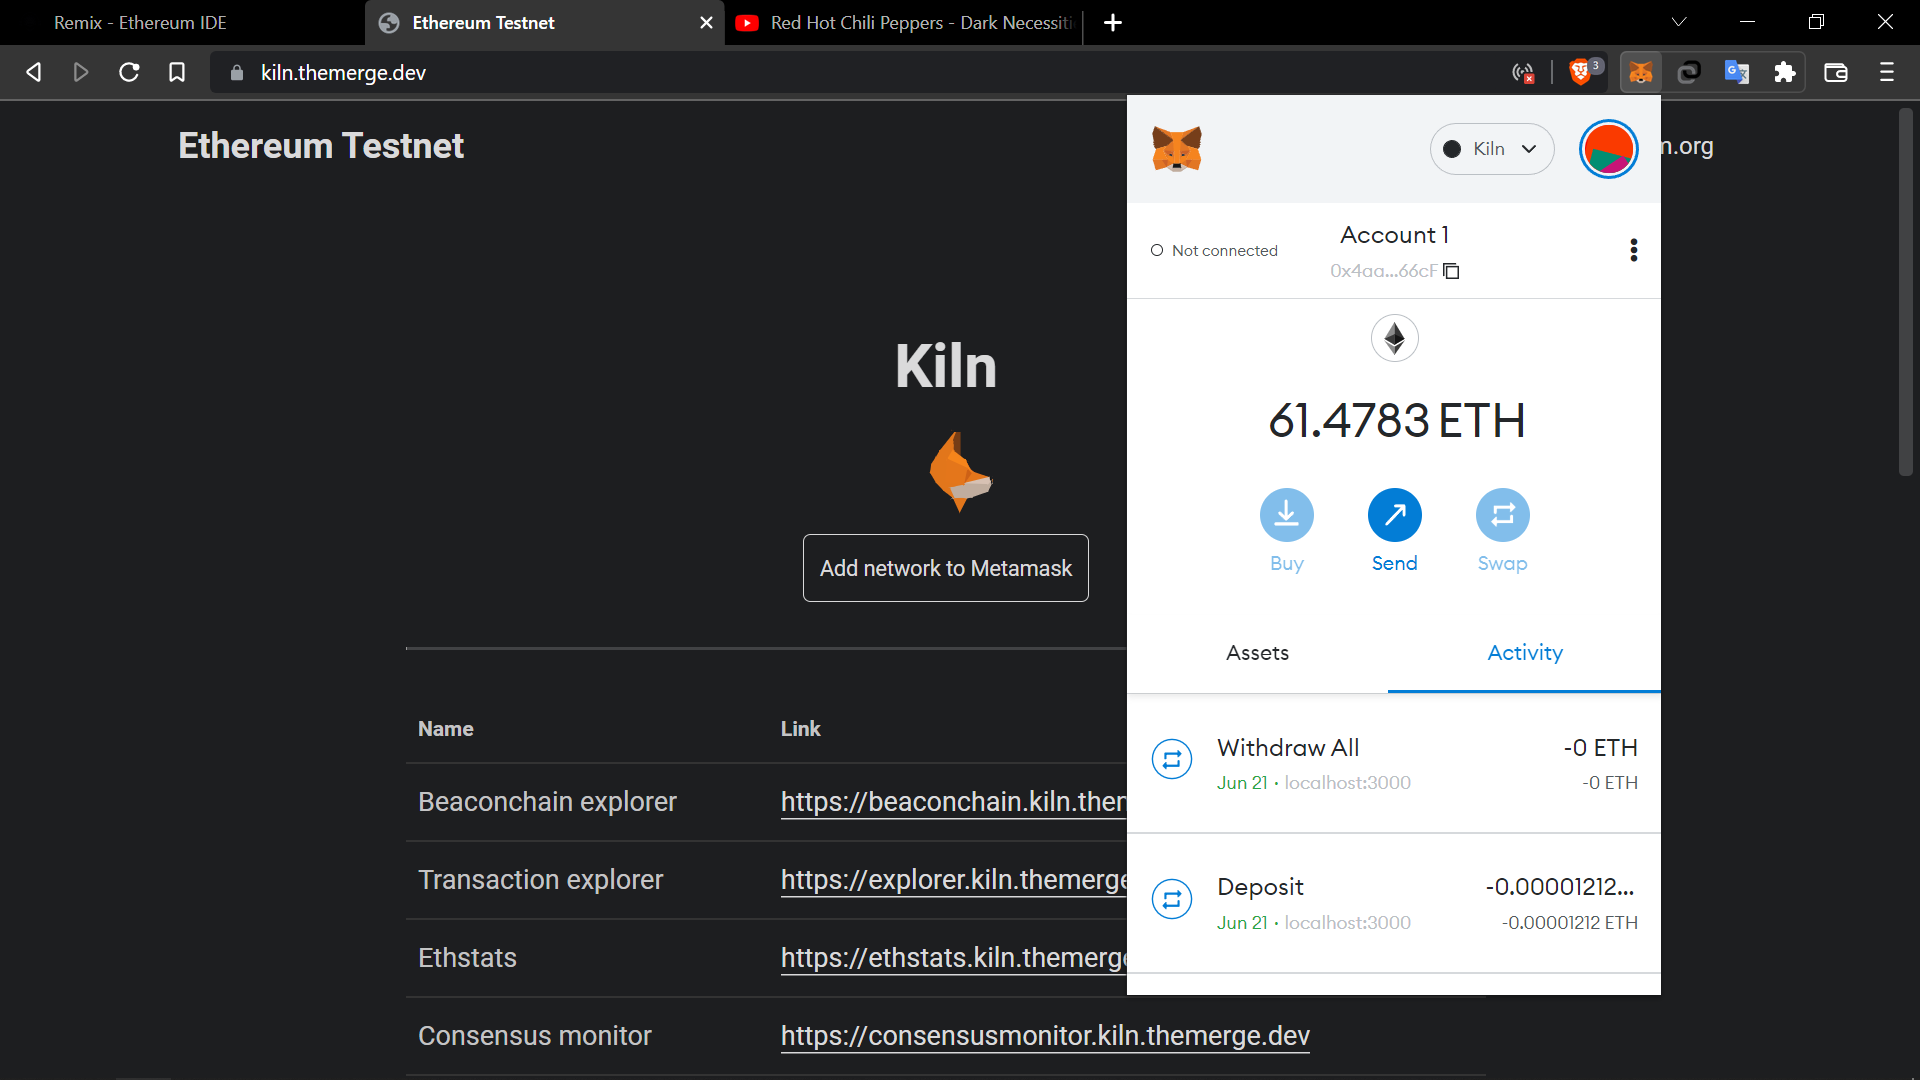
\includegraphics[scale=0.2]{gambar/bab3/metamask/6.png}
		\caption{Metamask siap digunakan}
		\label{fig:accready}
	\end{figure}
\end{enumerate}

\subsection{Frontend/Antarmuka User}
\label{subsec:frontenduser}

Bagian frontend atau biasa dikenal sebagai antarmuka user pada penelitian ini adalah bagian antarmuka tempat user melakukan berbagai interaksi dengan Smart Contract. Ada banyak library maupun framework yang tersedia untuk digunakan sebagai alat untuk membuat antarmuka user berbasis web ini. Salah satu library yang digunakan untuk pembuatan antarmuka user adalah Web3 JavaScript. Web3 JavaScript adalah sebuah API yang digunakan sebagai penghubung antara frontend web dengan smart contract. Web3 ini memungkinkan interaksi dengan smart contract pada pelbagai level dan mengirimkan hasil dari interaksi dengan smart contract dalam bentuk .json ke frontend. Pada Web3 secara umum, mempunyai beberapa fitur dasar untuk menghubungkan ke smart contract yang telah dibuat. Fitur tersebut adalah membuat module untuk Ethereum yang kita pilih, menginisiasi gateway yang digunakan, hingga melakukan transaksi blockchain secara umum.\\
Dalam pembuatan antarmuka untuk user, digunakan Web3 JavaScript untuk menghubungkan antara Smart Contract dengan antarmuka user. Untuk skema pengiriman data ke Smart Contract, frontend menggunakan yaitu Application Binary Interface. Application Binary Interface adalah sebuah interface antara frontend dengan setiap fungsi yang bisa diinteraksikan dalam suatu Smart Contract. ABI ini berberntuk JSON dengan memuat :
\begin{enumerate}
\item{Tipe. Yaitu golongan suatu fungsi bisa berupa 'fungsi','konstruktor', maupun 'terima'}
\item{Nama dari fungsi itu sendiri}
\item{Input yang diterima, baik parameter input maupun tipe input}
\item{Output yang akan dikeluarkan, setiap jenis maupun namanya}
\item{Kendali mutasi dari suatu fungsi. Yaitu kendali yang diberikan untuk berinteraksi mengubah satu maupun lebih variabel dalam suatu fungsi} 
\end{enumerate}
\newpage
Dari ABI ini, kemudian dibuatkan setiap fungsi javascript yang memanggil setiap fungsi yang bisa diinteraksikan. Telah dilakukan pembuatan ABI ke dalam JavaScript. Berikut hasilnya :
	
\begin{figure}[htp]
		\centering
		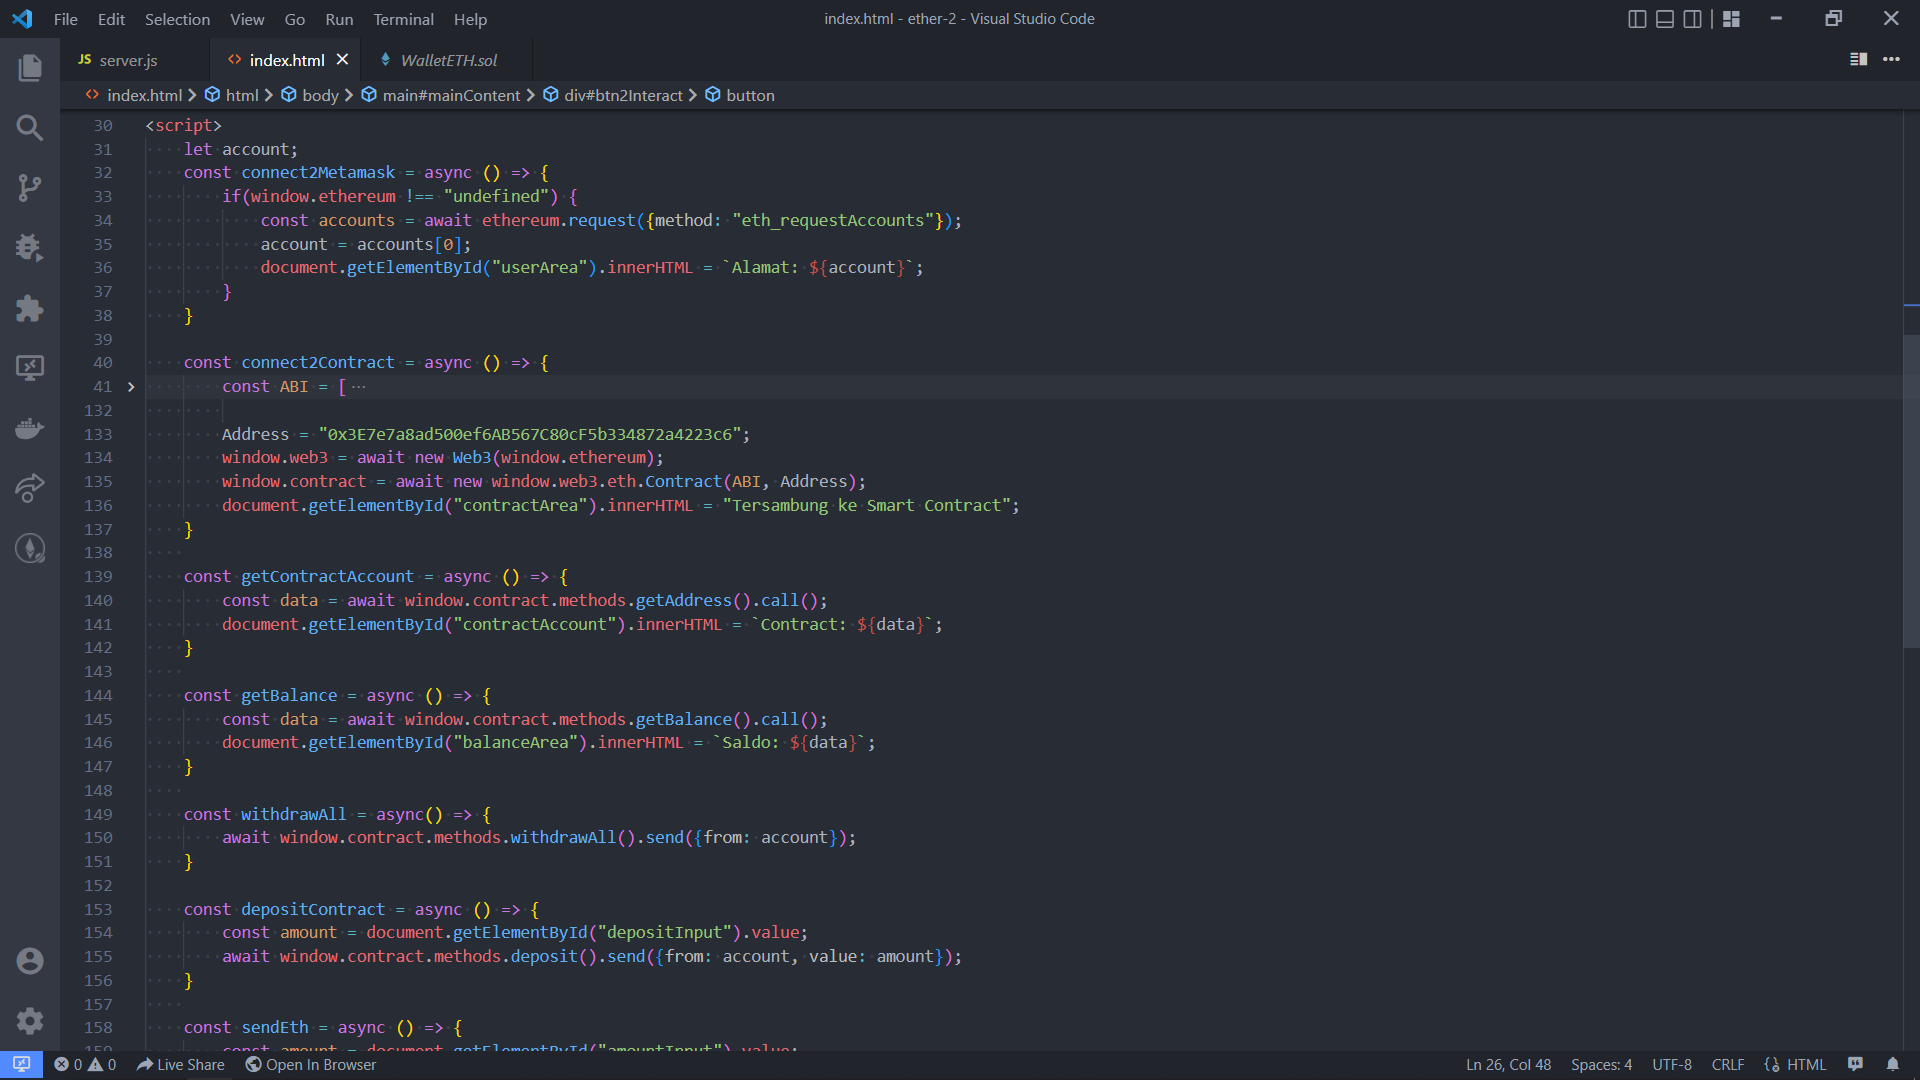
\includegraphics[scale=0.2]{gambar/bab3/front/1.png}
		\caption{Membuat variabel ABI ke dalam frontend (1)}
		\label{fig:abiready}
	\end{figure}

\begin{figure}[htp]
		\centering
		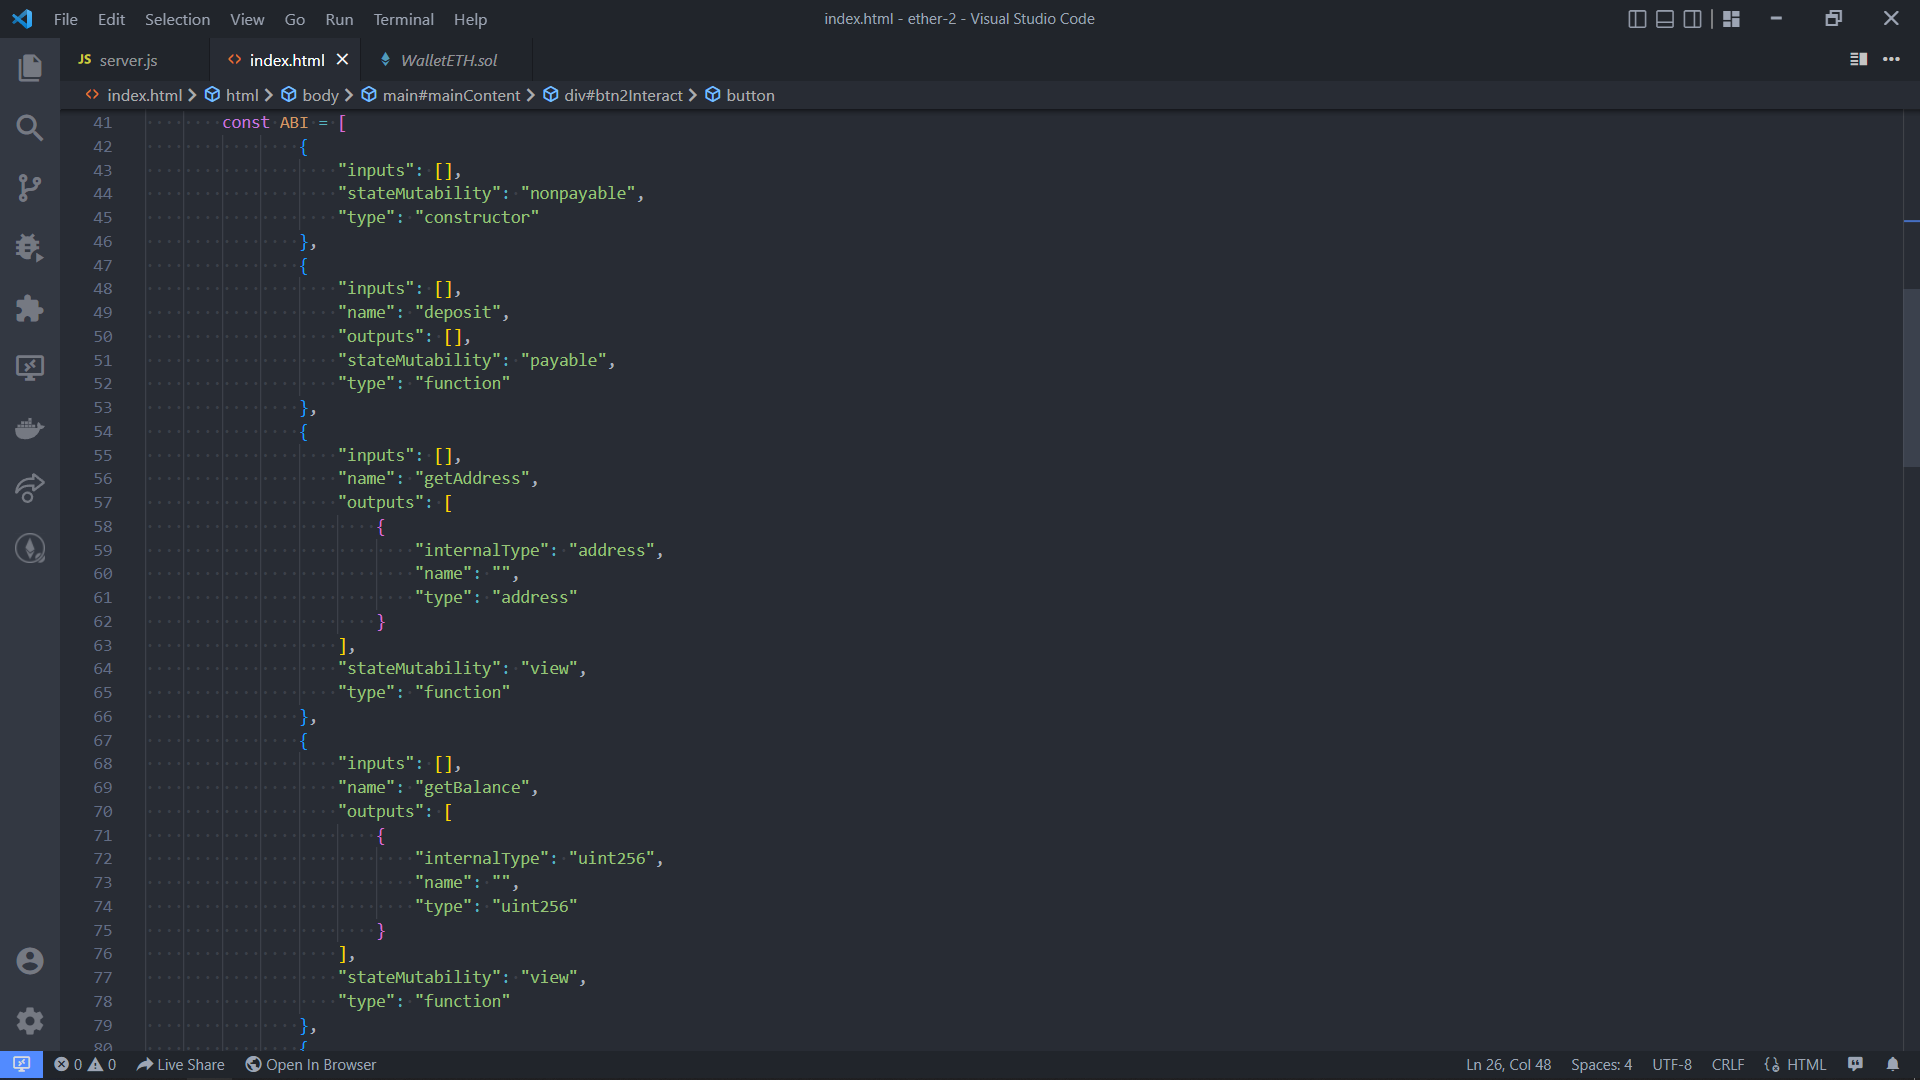
\includegraphics[scale=0.2]{gambar/bab3/front/2.png}
		\caption{Membuat variabel ABI ke dalam frontend (2)}
		\label{fig:abiready2}
	\end{figure}
\newpage
\section{Use Case User}
\label{sec:usecaseuser}

Di bagian antarmuka pengguna, ada beberapa fungsi utama dari penelitian ini yang bisa dilakukan oleh pengguna. Berikut adalah use case dari penggua.
\begin{figure}[htp]
	\centering
	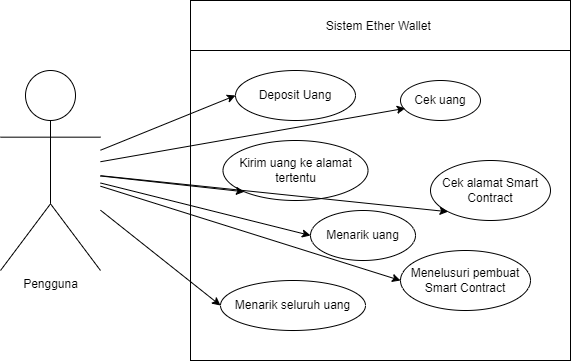
\includegraphics[scale=0.45]{gambar/use-case-diagram-sistem.png}
	\caption{Use Case Diagram antarmuka pengguna}
	\label{fig:usecasefrontend}
\end{figure}

Dari use case diagram diatas, fitur pengguna dapat dijabarkan menjadi berikut:

\begin{itemize}

\item{Deposit Uang}
	\\Deposit uang dari pengguna ke Smart Contract bisa dilakukan melalui gateway Ethereum. Deposit ini menggunakan satuan turunan Ether yaitu Wei. Deposit ke Smart Contract dilakukan untuk menggunakan fitur fitur yang tersedia di Smart Contract ini. Untuk melakukan fitur deposit pengguna bisa mengikut langkah berikut:
\begin{figure}[htp]
	\centering
	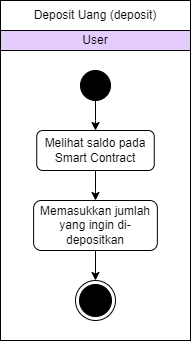
\includegraphics[scale=0.6]{gambar/deposit-diagram.png}
	\caption{Diagram cara deposit}
	\label{fig:diagramdeposit}
\end{figure}

\item{Mengambil Uang}
	\\Untuk fitur mengambil uang, pengguna diberikan dua opsi. Opsi pertama yaitu opsi utnuk mengambil sebagian uang yang telah dideposit ke Smart Contract. Opsi pertama menawarkan berapa banyak uang yang ingin diambil dalam satuan Wei.

\begin{figure}[htp]
	\centering
	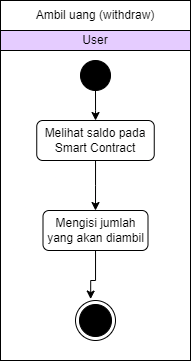
\includegraphics[scale=0.5]{gambar/withdraw-diagram.png}
	\caption{Diagram cara ambil sebagian uang dari Smart Contract}
	\label{fig:diagramwithdraw}
\end{figure}

Untuk fitur kedua yaitu opsi untuk mengambil seluruh uang yang telah dideposikan ke Smart Contract. Opsi ini memungkinkan seluruh uang yang telah dideposit diambil langsung.
\begin{figure}[htp]
	\centering
	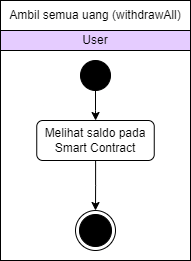
\includegraphics[scale=0.6]{gambar/withdrawAll-diagram.png}
	\caption{Diagram cara ambil seluruh saldo dari Smart Contract}
	\label{fig:diagramwithdrawall}
\end{figure}

\item{Mengirim Uang}
	\\Opsi mengirimkan uang yang telah disimpan di Smart Contract bisa dilakukan dengan mengisi alamat tujuan dan nominal yang dikirimkan dalam satuan Wei:
\begin{figure}[htp]
	\centering
	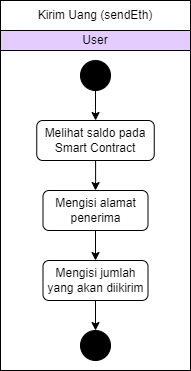
\includegraphics[scale=0.6]{gambar/sendEth-diagram.png}
	\caption{Diagram cara mengirim uang}
	\label{fig:diagramsendeth}
\end{figure}
\end{itemize}
